% Glava dokumenta
\documentclass[slovene, usenames,dvipsnames]{beamer}
\usepackage[utf8x]{inputenc}
\usepackage{lmodern}
\usepackage[T1]{fontenc}

% usetheme is the same as usepackage
% it just automatically prepends the 'beamertheme'
%\usetheme[]{progressbar}
\usefonttheme{progressbar}
\useoutertheme{progressbar}
\useinnertheme{progressbar}
\progressbaroptions{ headline=sections, titlepage=normal, frametitle=normal}
\usecolortheme{seahorse}
%\usecolortheme{progressbar}

% \usetheme[sectionpage=none, subsectionpage=none, numbering=none, progressbar=frametitle]{metropolis} % izbira nastavitev oblike in barv strani
%\usecolortheme{seahorse}
\usepackage{tikz}
\usepackage[slovene]{babel}
%\usetikzlibrary{arrows}
\usepgflibrary{arrows}% for more options on arrows
\usetikzlibrary{arrows.meta}
\usetikzlibrary{positioning}
\usepackage{varwidth}
\usepackage{color}
\usepackage{amsmath}
\usepackage{amsthm}
\usepackage{xcolor}
\usepackage{enumerate}
\usepackage{braket}
%\setbeamercolor{frametitle}{
%  use=palette primary,
%  bg=RoyalBlue}

%\setbeamercolor{background canvas}{
% use=palette primary,
% bg=White}

%\setbeamercolor{progress bar}{
%  fg=Blue}

%\setbeamercolor{progress bar in head/foot}{
%  fg=Red}

\usepackage{varwidth}
\setlength{\abovedisplayskip}{0pt}
\setlength{\belowdisplayskip}{0pt}


\uselanguage{slovene}
\languagepath{slovene}
\deftranslation[to=slovene]{Definition}{Definicija}
\usepackage{outlines}
\usepackage[document]{ragged2e}
\usepackage[customcolors,norndcorners]{hf-tikz}
\usetikzlibrary{calc} %% added

\graphicspath{{./slike/}{../slike/}{../eps_pdf/}}
\DeclareGraphicsExtensions{.eps,.jpeg,.png,.gif,.pdf}
\usepackage[outdir=../uporabljene_slike/]{epstopdf}
\epstopdfsetup{
	suffix=,
}

\newcommand{\Alpha}{A}
\newcommand{\Beta}{B}
\newcommand{\Epsilon}{E}
\newcommand{\Kappa}{K}
\newcommand{\dif}{\mathrm{d}}

\setbeamertemplate{navigation symbols}{}
\setbeamertemplate{section in toc}[sections numbered]
\setbeamertemplate{subsection in toc}[subsections numbered]

\setlength{\abovedisplayskip}{0pt}
\setlength{\abovedisplayshortskip}{0pt}
\setlength{\belowdisplayskip}{0pt}
\setlength{\belowdisplayshortskip}{0pt}

% this is from
% https://tex.stackexchange.com/questions/66125/extract-x-value-from-coordinate-in-tikz
\newdimen\XCoord
\newdimen\YCoord
\newcommand*{\ExtractCoordinate}[1]{\path (#1); \pgfgetlastxy{\XCoord}{\YCoord};}%


\author{Jure Lapajne}
\title{Calculation of nmr parameters in paramagnetic metal-organic materials}

\begin{document}
\titlepage

\begin{frame}{Presentation plan}
  \begin{enumerate}
  \item MOFs = Metal---organic frameworks \pause
  \item NMR --- what and why \pause
  \item NMR parameter calculation \pause
  \item DFT \pause
  \item Preliminary results
  \end{enumerate}
\end{frame}

\section{MOFs}
\begin{frame}{MOF = METAL-ORGANIC FRAMEWORK }
  \begin{minipage}[]{0.5\textwidth}
    \begin{itemize}[]
      \onslide<2-> \item crystal structure: central metallic ions + organic ligands 
      \onslide<3-> \item diversity: large number of possible combinations  
      \onslide<4-> \item wide usage: gas storage, clean energy applications,
      nonlinear optics, catalysts
      \onslide<5-> \item metallic ions commonly feature unpaired electrons
      \onslide<6-> \item NMR spectra feature large shifts caused by unpaired electrons
    \end{itemize}
  \end{minipage}%
\onslide<2->  \begin{minipage}[]{0.5\textwidth}
    \begin{minipage}[]{\textwidth}
      \centering
      \vspace{-0.5cm}
      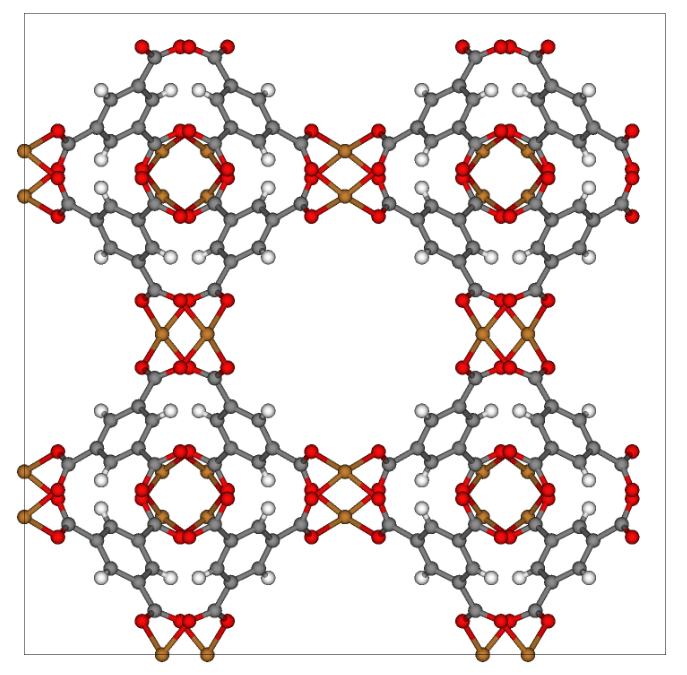
\includegraphics[width=0.7\textwidth]{hkust.png}
    \end{minipage}
    
    \begin{minipage}[]{\textwidth}
      \centering
      
\begin{tikzpicture}[remember picture,overlay]
      
        \def \dx {-1.2cm}
        \def \dy {-0.2cm}
        \def \Sdim {0.2cm}
        \definecolor{FillColor1}{RGB}{102,178,255};
        \definecolor{FillColor1}{RGB}{102,178,255};
        \def \ygap {0.5cm}
        \def \xgap {1.5cm}
        \def \radius {0.07}

        \draw [fill=black, thick, fill opacity=0.5] ($(\dx, \dy)$) circle [radius=\radius] node[right, black] {C};
     
        \draw [fill=red, red, thick] ($(\dx, \dy) + (0, -\ygap)$) circle [radius=\radius] node[right, black, align=center] {O};

        \draw [fill=brown, thick, orange] ($(\dx, \dy) + (\xgap,  0.0)$) circle [radius=\radius] node[right, black] {Cu};

        \draw [thick, draw=black, fill=white] ($(\dx, \dy) + (\xgap, -\ygap)$) circle [radius=\radius] node[right, black] {H};
      \end{tikzpicture}
    \end{minipage}
  \end{minipage}  
\end{frame}

\begin{frame}{NMR spectra of MOFs}
  \begin{itemize}
  \item usual organic molecules display shifts in range $[-200, 200]$ ppm
  \item MOF spectra display large shifts rarely seen in purely organic molecules  
  \end{itemize}
  \begin{minipage}[]{0.6\textwidth}
    \hspace{1cm}
      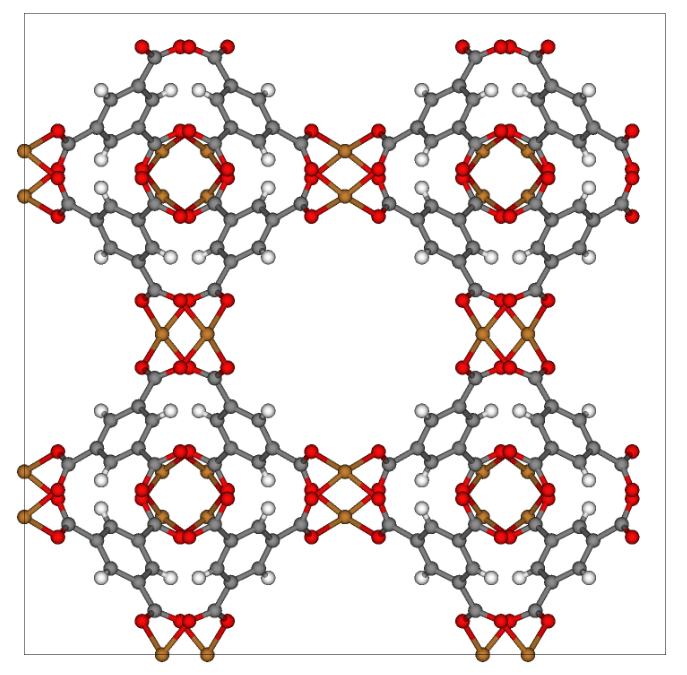
\includegraphics[width=0.7\textwidth]{hkust.png}
           \begin{tikzpicture}[remember picture,overlay]

      \def \center {current page.center};
      \coordinate (number1) at ($(current page.center)-(-0.34, 0.95)$);
      \coordinate (number2) at ($(number1)-(0, 0.35)$);
      \coordinate (number3) at ($(number1)-(0, 0.7)$);

      \coordinate (atom_pos1) at ($(number1) + (-0.91, 0.16)$);
      \coordinate (atom_pos2) at ($(number2) + (-0.8, 0.64)$);
      \coordinate (atom_pos3) at ($(number3) + (-1.05, 0.7)$);
      
 % \coordinate (arrow1) at ($ (\xArrowCenter, \yArrowCenter) +  (-0.5,-0.2) $);
      \node[red] at (number1) (atom1) {1};
      \node[blue] at (number2) (atom2) {2};
      \node[green] at (number3) (atom3) {3};
      
      \draw[red] (atom_pos1) -- ($(number1) - (0.1, 0)$) ;
      \draw[blue] (atom_pos2) -- ($(number2) - (0.1, 0)$);
      \draw[green] (atom_pos3) -- ($(number3) - (0.1, 0)$);
    \end{tikzpicture}
  \end{minipage}%
  \begin{minipage}[]{0.4\textwidth}
    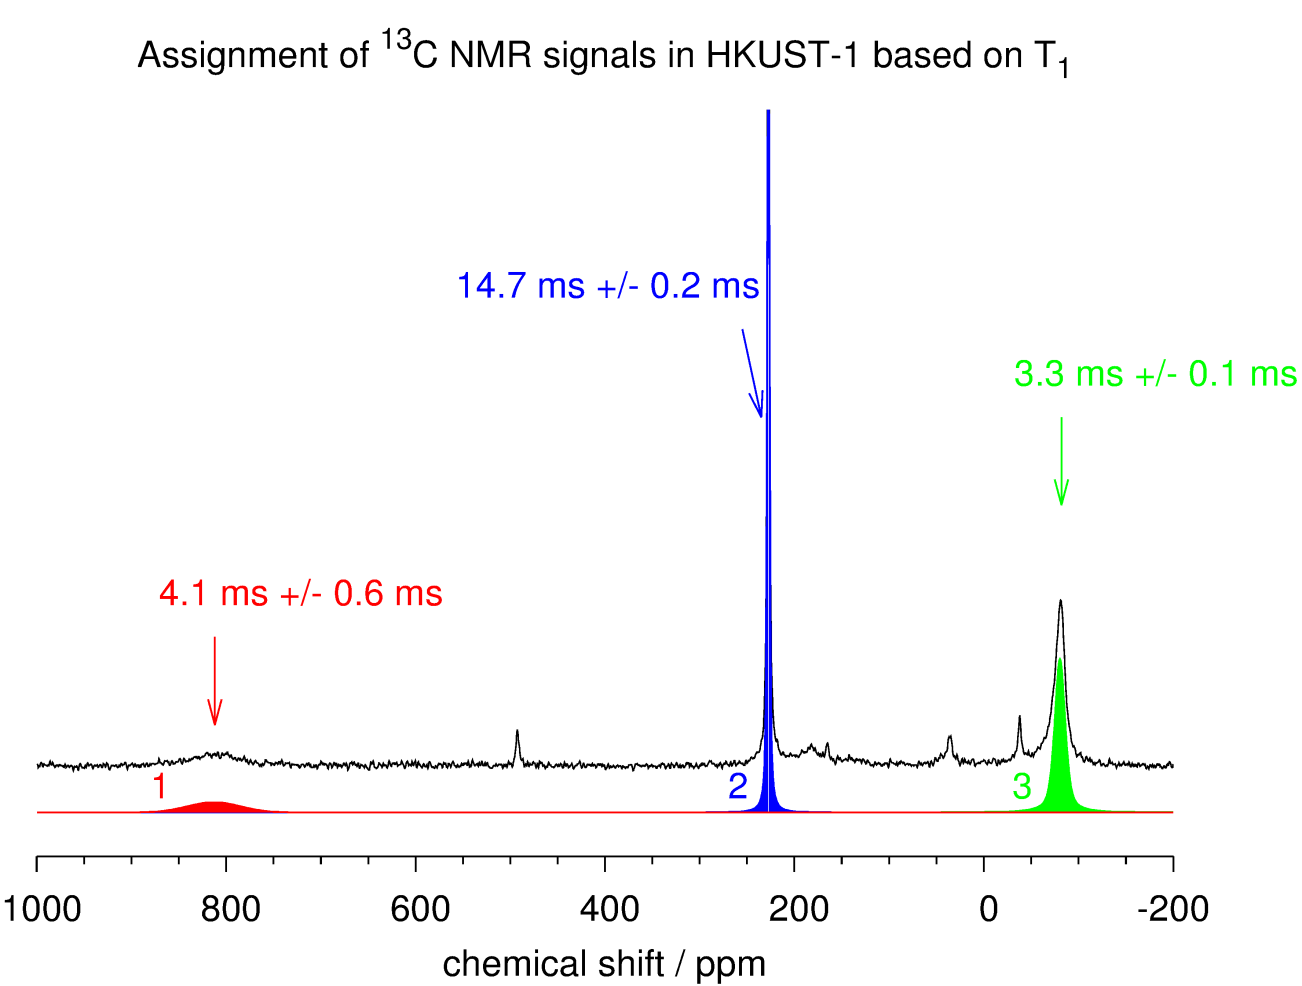
\includegraphics[width=0.9\textwidth]{hkust_spekter.png}
  \end{minipage}
  \end{frame}

\section{NMR}
\begin{frame}{Nuclei in external magnetic field}
  \begin{itemize}[]
  \onslide<2-> \item strong external magnetic field: several T
  \onslide<3->\item nuclei with magnetic moment: lowest energy state splits
  \onslide<4->  \item two new states $\Delta E$ apart
  \onslide<5-> \item radio frequency spectrum: excitations from low to high energy states
  \onslide<6-> \item absorption peak at $\Delta E=\hbar \omega_{res}$
    \item $\omega_{res}$ depends on $B_{eff}(observed nucleus)$
    \end{itemize}
    \onslide<3->   \begin{minipage}[]{\textwidth}
      \centering
    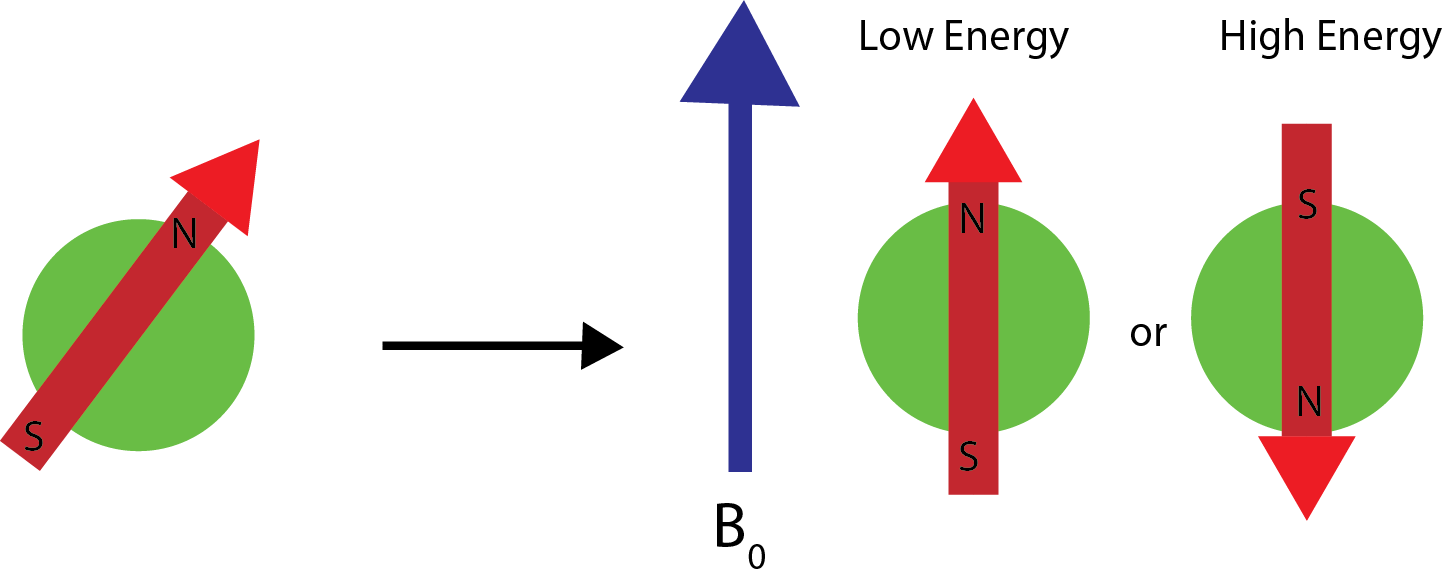
\includegraphics[width=0.5\textwidth]{spin_energy_states.png}
\end{minipage}
\end{frame}


\begin{frame}{Effective magnetic field}
  Several parameters affect $B_{eff}(nucleus)$ and $\omega_{res}$: \pause
  \begin{itemize}[]
  \item electronic structure -- shielding of external magnetic field \pause 
  \item spin--spin coupling to nearby nuclei and unpaired electrons \pause
  \item unpaired electrons: large paramagnetic shifts \pause
    \item calculation of nmr parameters: accurate knowledge of electronic wavefunction
   \end{itemize}
 \begin{minipage}[]{0.4\textwidth}
      \centering
    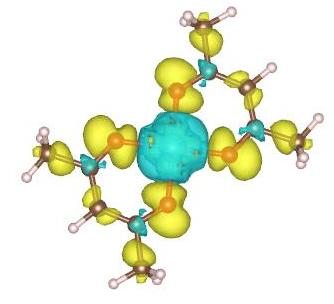
\includegraphics[width=0.8\textwidth]{cuacac_spin_density.png}
 \end{minipage}%
 \begin{minipage}[]{0.6\textwidth}
   \centering
    \begin{itemize}[]
    \item MOFs: metal-organic frameworks \pause
    \item transition metal atoms: unpaired electrons \pause
   \end{itemize}
 \end{minipage}
\end{frame}


\begin{frame}{Chemical and hyperfine shifts}

     \onslide<2->    \begin{definition}
 Total shift tensor $\underline{\underline{\sigma}}$ is defined by:
        \vspace*{-0.5\baselineskip}
        \centering
    \begin{equation} \nonumber
      \vec{B}_{eff}=\vec{B}_0\left( \underline{\underline{ \mathrm I }} - \underline{\underline{ \sigma}} \right).
    \end{equation}
  \end{definition}

  \centering Two sources of chemical shifts:
  
  \begin{minipage}[t]{0.5\textwidth}
    \begin{itemize}[]
    \onslide<3-> \item electron density change caused by applied external magnetic field
    \onslide<3-> \item depends on electron density $n(\vec r)$
      \end{itemize}
  \end{minipage}%
  \begin{minipage}[t]{0.5\textwidth}
    \begin{itemize}[]
    \onslide<3->  \item coupling between unpaired electron and observed nuclei
    \onslide<3-> \item depends on spin density $n_{\uparrow}(\vec r_{nuclei}) - n_{\downarrow}(\vec r_{nuclei})$
      \end{itemize}
    \end{minipage}
    Calculation of NMR parameters:\\ \bf{accurate electronic wave function needed!}
  \end{frame}

  \section{DFT}

  
  \begin{frame}{electronic wave function calculation}
  \onslide<2->  \begin{equation}\nonumber
      \hat H = T_n + T_e + W_{n-n} +  W_{e-n} + W_{e-e} +V_{ext}
    \end{equation}
    \begin{itemize}[]
    \onslide<3->\item Born-Oppenheimer approximation
    \onslide<4->\item direct solution of coupled pde not feasible
    \onslide<5->\item given accuracy level: time grows exponentially as a function of number of particles
    \\
    \onslide<6-> \centering Approximations
    \\
    \begin{minipage}[t]{0.5\textwidth}

     \onslide<7->  \centering  DFT
      \begin{itemize}
      \onslide<8->\item most widely used
      \onslide<9->\item good tradeoff between accuracy and speed
      \onslide<10-> \item highly customizable - suitable for various molecules
      \end{itemize}      
    \end{minipage}%
    \begin{minipage}[t]{0.1\textwidth}
      \end{minipage}%
    \begin{minipage}[t]{0.4\textwidth}
      \onslide<11-> \centering  Alternatives
      \begin{enumerate}[$\ast$]
      \onslide<12->\item Hartree---Fock
      \onslide<13->\item Quantum Monte Carlo
      \onslide<14->\item Coupled-Cluster methods
      \end{enumerate}
      \centering  $\vdots$
    \end{minipage}
    \end{itemize}
    
\onslide<3-> \begin{tikzpicture}[remember picture,overlay]

      \def \center {current page.center};
      \coordinate (center1) at ($(\center) + (-2.9cm, 2.25cm)$);
      \coordinate (start1) at ($(center1) + 0.5*(0cm, -1cm)$);
      \coordinate (end1) at ($(center1) + 0.5*(1cm, -2cm)$);

      \coordinate (center2) at ($(\center) + (-1.05cm, 2.3cm)$);
      \coordinate (start2) at ($(center2) + 0.6*(0cm, -1cm)$);
      \coordinate (end2) at ($(center2) + 0.53*(1cm, -2cm)$);
 % \coordinate (arrow1) at ($ (\xArrowCenter, \yArrowCenter) +  (-0.5,-0.2) $);
    	\draw  [thick, red] (start1) -- (end1);
      \draw  [thick, red] (start2) -- (end2);
    \end{tikzpicture}
  \end{frame}

  
  \begin{frame}{density functional theory --- DFT}
    \begin{minipage}[]{\textwidth}
      $N$-particle problem:
      \begin{itemize}
      \item DFT effectively reduces $N$-particle problem to 1-particle problem
      \item Kohn-Sham theorems: transition from $3N$ to $3$ coordinates.
      \end{itemize}
    \end{minipage}
    \begin{minipage}[]{\textwidth}
      \centering
      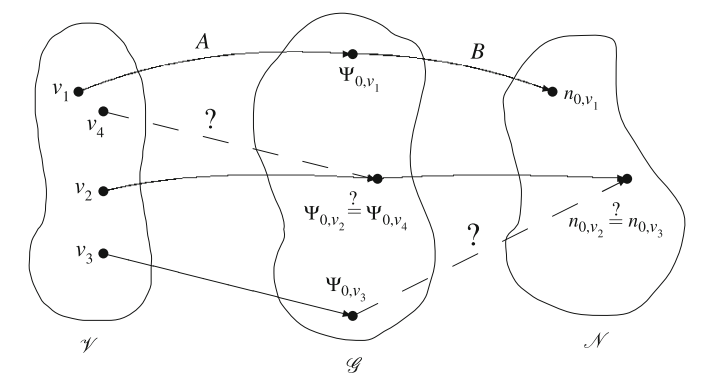
\includegraphics[width=0.5\textwidth]{bijekcija_med_v_psi_n.png}
    \end{minipage}
    System of $N$--particles:
    \begin{itemize}
    \item bijection between the set of external potentials and corresponding
      non-degenerate ground states
    \item bijection between the set of ground states and the set of ground
      states electron densities
    \end{itemize}

  \end{frame}
  
  \begin{frame}{energy as a functional of density}
      \centering
      \onslide<2->  Ground state $\ket{\psi_0}$:
      \onslide<3->  \begin{equation} \nonumber
        \hat H \ket{\psi_0} =E_0\ket{ \psi_0},\quad \mathrm{with}
        \quad \braket{\psi_0|\psi_0}=1.
      \end{equation}
      \onslide<4->    Using bijection from previous slide, one can write:
      \onslide<5->       \begin{equation} \nonumber
        \ket{\psi_0}=\ket{\Psi_0[n_0(\vec r)]},
      \end{equation}
      \onslide<6->  and
      \begin{equation} \nonumber
        E_0[n_0(\vec r)]=\braket{\Psi[n_0(\vec r)]|\hat H|\Psi[n_0(\vec r)]}.
      \end{equation}
    \centering
    \onslide<7->  Unfortunately the functional $\Psi[n_0(\vec r)]$ not known!
    \\
    \onslide<8->   $E[n(\vec r)]$ is modelled emperically.
  \end{frame}

  \begin{frame}{Energy functional}
    \centering $E[n(\vec r)]$ should contain:
\\    
    \begin{minipage}[t]{0.45\textwidth}
      \begin{enumerate}[$\ast$]
      \item kinetic energy $T[n(\vec r)]$
      \item coulomb interaction
        \begin{equation}\nonumber
             E_H[n] = \frac{1}{2}\int \frac{n(\vec r)n(\vec {r'})}{|\vec r - \vec r'|} \dif \vec r  \dif \vec r'
        \end{equation}
      \end{enumerate}
    \end{minipage}%
    \begin{minipage}[t]{0.55\textwidth}
      \begin{enumerate}[$\ast$]
      \item exchange -- correlation term $E_{xc}[n(\vec r)]$
      \item external potential
        \begin{equation}\nonumber
          \hspace{-1cm}
          V_{ext}[n] = \frac{1}{2}\int n(\vec r) v_{ext}(\vec r)\dif \vec r
      \end{equation}
    \end{enumerate}
    \vspace{0.2cm}
  \end{minipage}
  
  \begin{minipage}[]{0.5\textwidth}
    Issues:
    \begin{itemize}
    \item kinetic energy term
    \item  Calculation on exchange-correlation part
      \end{itemize}
    \end{minipage}%
      \begin{minipage}[]{0.5\textwidth}
    Solution:
    \begin{itemize}
    \item use of Slater determinant
    \item  various approaches, no general rule/solution
      \end{itemize}
    \end{minipage}
  \end{frame}


  \begin{frame}{Calculation procedure}
 
    \begin{tikzpicture}[remember picture,overlay]
      
      \def \dx {-1.2cm}
      \def \dy {-0.2cm}
      \def \Sdim {0.2cm}
      \definecolor{FillColor1}{RGB}{102,178,255};
      \definecolor{FillColor1}{RGB}{102,178,255};
      \def \ygap {0.5cm}
      \def \xgap {1.5cm}
      \def \radius {0.07cm}

      
      \onslide <2-> \node at ($(current page.center) + (0, 2.6cm)$)
      [rectangle,draw] (equation1) {Construct potential of nuclei and
        include it in $V_{ext}(\vec r)$.};

      \onslide <3->  \node at ($(current page.center) + (0, 1.3cm)$)
      [rectangle,draw] (equation2) {Compute $E_{H}[n(\vec r)]$,
        $E_{xc}[n(\vec r)]$ and $E_{ext}[n(\vec r)]$};
      
      \onslide <4->  \node at (current page.center) [rectangle,draw] (equation3)
      {solve $\left(T[n(\vec r)]+E_{H}[n(\vec r)]+E_{xc}[n(\vec r)]+
          E_{ext}[n(\vec r)]\right)\psi_i=\epsilon_i\psi_i$};

      \onslide <5->  \node at  ($(current page.center) + (0, -1.3cm)$)
      [rectangle,draw] (equation4)  {compute $n(\vec r)=\sum_{i}\psi_i$,
         where $\epsilon_i<\epsilon_f$};
      
       \onslide <6->  \node at  ($(current page.center) + (0, -2.6cm)$)
       [rectangle,draw] (equation5) {check convergence of $\epsilon_i$ and
         $n(\vec r)$};

       \onslide <8->  \node at  ($(current page.center) + (0, -3.9cm)$)
       [rectangle,draw] (equation6)  {calculate energy and forces};

       \onslide <3-> \draw [->, thick, black]
       (equation1.south) -- (equation2.north);

       \onslide <4->\draw [->, thick, black]
       (equation2.south) -- (equation3.north);

       \onslide <5-> \draw [->, thick, black]
       (equation3.south) -- (equation4.north);

       \onslide <6-> \draw [->, thick, black]
       (equation4.south) -- (equation5.north);

       \onslide <8-> \draw [->, thick, black]
       (equation5.south) -- (equation6.north)
       node[right, yshift=0.3cm] {converged};

       \onslide <7-> \draw [ thick, black]
       (equation5.west) -- ($(equation5.west)+(-2.8 , 0)$)
       node[align=center, above, xshift=1 cm] {not}
       node[align=center, below, xshift=1 cm] {converged};


       \path let \p1 = (equation2.west) in coordinate (temp1) at (0, \y1);
       \path let \p1 = (equation5.west) in coordinate (temp2) at ( \x1,0);
       
       \ExtractCoordinate{equation5.west}
       \onslide <7-> \draw [->, thick, black]
       ($(equation5.west)+(-2.8 , 0)$) --
        ($(temp1)+(temp2)+(-2.8,0)$) --
       ($(equation2.west)+(0 , 0)$);

       \path let \p1 = (equation1.east) in coordinate (temp1) at (0, \y1);
       \path let \p1 = (equation6.east) in coordinate (temp2) at ( \x1,0);
       \onslide <9-> \draw [->, thick, black]
       ($(equation6.east)+(3.5 , 0)$) --
       ($(temp1)+(temp2)+(3.5, 0)$) --
       ($(equation1.east)$);

        \onslide <9-> \draw [ thick, black]
        (equation6.east) -- ($(equation6.east)+(3.5 , 0)$)
        node[align=center, above, xshift = -1.75 cm] {move nuclei};
      
      \end{tikzpicture}
    \end{frame}

    \begin{frame}{DFT flexibility}
      \begin{minipage}[]{0.6\textwidth}
      Large number of various exchange-correlation functionals:
      \begin{itemize}
      \item hybrid: GGA + hartree-fock exchange
                \scriptsize
        $-\frac{1}{2}\sum_{k,l}\int \frac{
          \phi^*_k(\vec r,
        \sigma)\phi_l(\vec{r}, \sigma)
        \phi^*_l(\vec{r'}, \sigma')\phi_k(\vec{r'}, \sigma')}{|\vec r - \vec
        r'|}
      \dif \vec{r} \dif \vec{r'}$
     \item meta--GGA: higher order derivatives
     \item GGA:  \small{$E_{xc}^{gga}=\int n(\vec r)^{4/3}F(|\nabla n(\vec
          r)|/n(\vec r)^{4/3})$}
      \item LDA: uniform gas \small{
          $E_{xc}^{lda}[n]=-C\int n(\vec r)^{4/3} \dif \vec r$}
      \end{itemize}
      \end{minipage}%
    \begin{minipage}[]{0.4\textwidth}
      \centering
      \vspace{-0.5cm}
      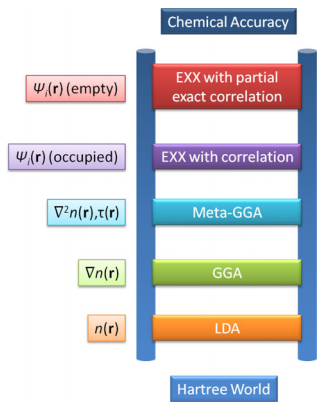
\includegraphics[width=0.7\textwidth]{jacobs_functional_ladder_ver2.png}
      \end{minipage}
      \end{frame}

      \begin{frame}{My work}
        \begin{minipage}[]{0.5\textwidth}
          \begin{itemize}
          \onslide <2->\item various functionals,
          \onslide <3->\item various basis sets,
          \onslide <4->\item boundary conditions: periodic vs single molecule,
          \onslide <5->\item full electron dft vs frozen core dft
          \end{itemize}
        \end{minipage}%
        \begin{minipage}[]{0.5\textwidth}
          \onslide <5-> 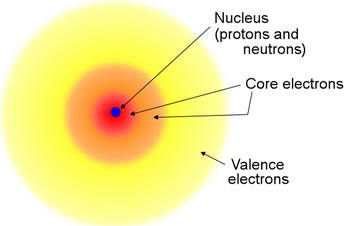
\includegraphics[width=0.5\textwidth]{valence_core_electrons.jpg}
          \onslide <5-> 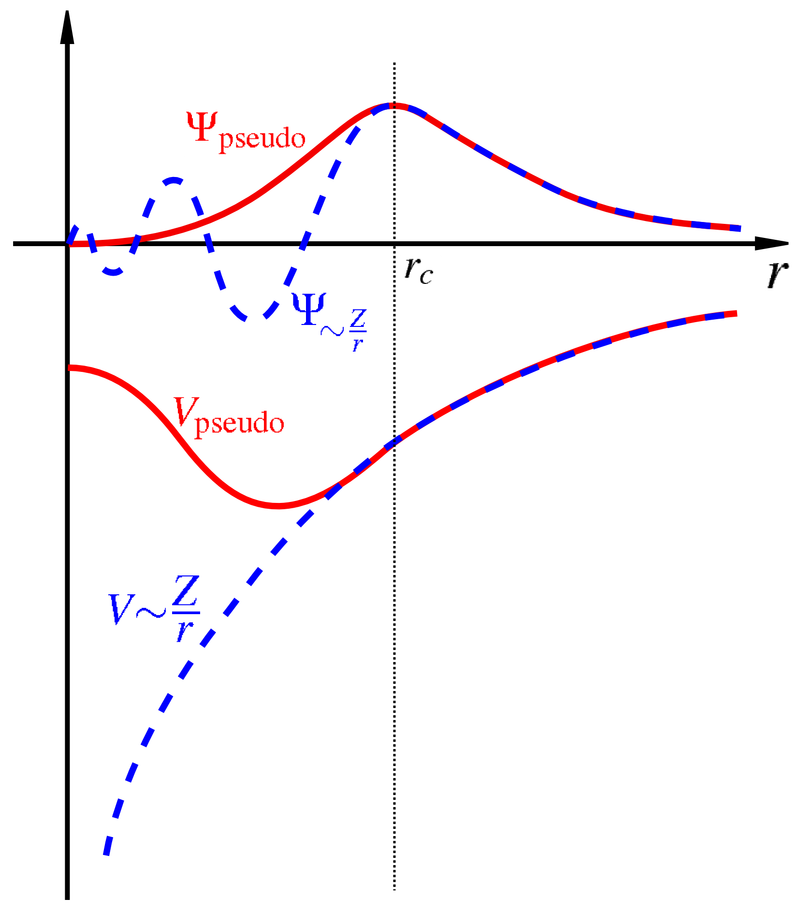
\includegraphics[width=0.5\textwidth]{pseudopotential.png}
          
        \end{minipage}
      \end{frame}
      
    \begin{frame}{Conclusion}
      \begin{enumerate}
        \item investigation of nmr
      \end{enumerate}
    \end{frame}

\end{document}